\documentclass[spanish,a4paper,11pt,twoside]{report}

%%%%%%%%%%%%%%%%%%%%%%%%%%%%%%%%%%%%%%%%%%%%%%%%%%%%%%%%%%%%%%%%%%%%%%%%%%%%%%%
\usepackage[dvips]{graphicx}
\usepackage[dvips]{epsfig}
\usepackage[latin1]{inputenc}
\usepackage[spanish]{babel}
\usepackage{alltt}
\usepackage{templates/algorithm}
\usepackage{templates/algorithmic}
\usepackage{templates/multirow}

%%%%%%%%%%%%%%%%%%%%%%%%%%%%%%%%%%%%%%%%%%%%%%%%%%%%%%%%%%%%%%%%%%%%%%%%%%%%%%%

\newcommand{\SONY}{{\sc Sony}}
\newcommand{\MICROSOFT}{{\sc Microsoft}}
\newcommand{\GCC}{\textsf{\textsc{G}CC}}
\newcommand{\INTEL}{\textsf{\textsc{I}ntel}}

%%% Traducimos el pseudocodigo
\renewcommand{\algorithmicwhile}{\textbf{mientras}}
\renewcommand{\algorithmicend}{\textbf{fin}}
\renewcommand{\algorithmicdo}{\textbf{hacer}}
\renewcommand{\algorithmicif}{\textbf{si}}
\renewcommand{\algorithmicthen}{\textbf{entonces}}
\renewcommand{\algorithmicrepeat}{\textbf{repetir}}
\renewcommand{\algorithmicuntil}{\textbf{hasta que}}
\renewcommand{\algorithmicelse}{\textbf{en otro caso}}
\renewcommand{\algorithmicfor}{\textbf{para}}

%\newcommand{\RETURN}{\textbf{retornar} }
\newcommand{\RET}{\STATE \textbf{retornar} }
\newcommand{\TO}{\textbf{hasta} }
\newcommand{\AND}{\textbf{y} }
\newcommand{\OR}{\textbf{o} }

%%%%%%%%%%%%%%%%% Creamos un entorno para listar c�digo fuente %%%%%%%%%%%%%%%
\newenvironment{sourcecode}
{\begin{list}{}{\setlength{\leftmargin}{1em}}\item\scriptsize\bfseries}
{\end{list}}

\newenvironment{littlesourcecode}
{\begin{list}{}{\setlength{\leftmargin}{1em}}\item\tiny\bfseries}
{\end{list}}

\newenvironment{summary}
{\par\noindent\begin{center}\textbf{Abstract}\end{center}\begin{itshape}\par\noindent}
{\end{itshape}}

\newenvironment{keywords}
{\begin{list}{}{\setlength{\leftmargin}{1em}}\item[\hskip\labelsep \bfseries Keywords:]}
{\end{list}}

\newenvironment{palabrasClave}
{\begin{list}{}{\setlength{\leftmargin}{1em}}\item[\hskip\labelsep \bfseries Palabras clave:]}
{\end{list}}


%%%%%%%%%%%%%%%%%%%%%%%%%%%%%%%%%%%%%%%%%%%%%%%%%%%%%%%%%%%%%%%%%%%%%%%%%%%%%%%
% Format
%%%%%%%%%%%%%%%%%%%%%%%%%%%%%%%%%%%%%%%%%%%%%%%%%%%%%%%%%%%%%%%%%%%%%%%%%%%%%%%

%%\topmargin -4 mm
%\topmargin -21 mm
%\headheight 10 mm
%\headsep 10 mm

%\textheight 229 mm
%\textheight 246 mm

%\oddsidemargin -5.4 mm
%\evensidemargin -5.4 mm
\oddsidemargin 5 mm
\evensidemargin 5 mm

%\oddsidemargin -3 mm
%\evensidemargin -3 mm

%\textwidth 17 cm
\textwidth 15 cm
%\columnsep 10 mm

\input{amssym.def}

%%%%%%%%%%%%%%%%%%%%%%%%%%%%%%%%%%%%%%%%%%%%%%%%%%%%%%%%%%%%%%%%%%%%%%%%%%%%%%%

\begin{document}

%%%%%%%%%%%%%%%%%%%%%%%%%%%%%%%%%%%%%%%%%%%%%%%%%%%%%%%%%%%%%%%%%%%%%%%%%%%%%%%
% First Page 
%%%%%%%%%%%%%%%%%%%%%%%%%%%%%%%%%%%%%%%%%%%%%%%%%%%%%%%%%%%%%%%%%%%%%%%%%%%%%%%

\pagestyle{empty}
\thispagestyle{empty}


\newcommand{\HRule}{\rule{\linewidth}{1mm}}
\setlength{\parindent}{0mm}
\setlength{\parskip}{0mm}
\vspace*{\stretch{1}}

\begin{center}

\includegraphics[width=0.2\textwidth]{images/logotipo-secundario-ULL}\\[0.25cm]
\end{center}

\HRule
\begin{center}
        {\Huge Obtenci�n de ra�ces} \\[2.5mm] 
        {\Huge M�todo de bisecci�n} \\[2.5mm]
        {\Large Claudia Ballester Niebla, Carlos Herrera Carballo, Cathaysa P�rez Quintero} \\[5mm]
        {\Large \textit{Grupo ($1\mid E$) }} \\[5mm]


        {\em T�cnicas Experimentales. $1^{er}$ curso. $2^{do}$ cuatrimestre} \\[5mm]
        Lenguajes y Sistemas Inform�ticos \\[5mm]
        Facultad de Matem�ticas \\[5mm]
        
        Universidad de La Laguna \\
\end{center}
\HRule
\vspace*{\stretch{2}}
\begin{center}
  La Laguna, \today 
\end{center}

%%%%%%%%%%%%%%%%%%%%%%%%%%%%%%%%%%%%%%%%%%%%%%%%%%%%%%%%%%%%%%%%%%%%%%%%%%%%%%%
\begin{abstract}
A lo largo de este informe se mostrar�n los experimentos realizados con el c�digo, implementado en Python, con el fin de encontrar las ra�ces de una funci�n,
a trav�s del m�todo de bisecci�n. As�, se podr�n encontrar los pasos seguidos para demostrar la eficacia del programa y las conclusiones obtenidas de los mismos.

Ser� posible acceder al c�digo implementado, y los datos recopilados en cada uno de los experimentos mencionados, adem�s de los antecedentes te�ricos, con sus
demostraciones correspondientes, que han servido para demostrar el m�todo utilizado para la obtenci�n de ra�ces. El m�todo de Bisecci�n.

\end{abstract}
%%%%%%%%%%%%%%%%%%%%%%%%%%%%%%%%%%%%%%%%%%%%%%%%%%%%%%%%%%%%%%%%%%%%%%%%%%%%%%%
\newpage{\pagestyle{empty}\cleardoublepage}

\pagestyle{myheadings} %my head defined by markboth or markright
% No funciona bien \markboth sin "twoside" en \documentclass, pero al
% ponerlo se dan un mont�n de errores de underfull \vbox, con lo que no se
% ha puesto.
\markboth{Nombre del alumno}{T�tulo del trabajo}

%%%%%%%%%%%%%%%%%%%%%%%%%%%%%%%%%%%%%%%%%%%%%%%%%%%%%%%%%%%%%%%%%%%%%%%%%%%%%%%
%Numeracion en romanos
\renewcommand{\thepage}{\roman{page}}
\setcounter{page}{1}

%%%%%%%%%%%%%%%%%%%%%%%%%%%%%%%%%%%%%%%%%%%%%%%%%%%%%%%%%%%%%%%%%%%%%%%%%%%%%%%

\tableofcontents

%%%%%%%%%%%%%%%%%%%%%%%%%%%%%%%%%%%%%%%%%%%%%%%%%%%%%%%%%%%%%%%%%%%%%%%%%%%%%%%
\newpage{\pagestyle{empty}\cleardoublepage}

\listoffigures

%%%%%%%%%%%%%%%%%%%%%%%%%%%%%%%%%%%%%%%%%%%%%%%%%%%%%%%%%%%%%%%%%%%%%%%%%%%%%%%
\newpage{\pagestyle{empty}\cleardoublepage}

\listoftables

%%%%%%%%%%%%%%%%%%%%%%%%%%%%%%%%%%%%%%%%%%%%%%%%%%%%%%%%%%%%%%%%%%%%%%%%%%%%%%%
\newpage{\pagestyle{empty}\cleardoublepage}

%%%%%%%%%%%%%%%%%%%%%%%%%%%%%%%%%%%%%%%%%%%%%%%%%%%%%%%%%%%%%%%%%%%%%%%%%%%%%%%
%Numeracion a partir del capitulo I
\renewcommand{\thepage}{\arabic{page}}
\setcounter{page}{1}

\setlength{\parindent}{5mm}

%%%%%%%%%%%%%%%%%%%%%%%%%%%%%%%%%%%%%%%%%%%%%%%%%%%%%%%%%%%%%%%%%%%%%%%%%%%%%%%
\chapter{Motivaci�n y objetivos}
\label{chapter:obj}

%%%%%%%%%%%%%%%%%%%%%%%%%%%%%%%%%%%%%%%%%%%%%%%%%%%%%%%%%%%%%%%%%%%%%%%%%%%%%
% Chapter 1: Motivaci�n y Objetivos 
%%%%%%%%%%%%%%%%%%%%%%%%%%%%%%%%%%%%%%%%%%%%%%%%%%%%%%%%%%%%%%%%%%%%%%%%%%%%%%%

Los objetivos le dan al lector las razones por las que se realiz� el
proyecto o trabajo de investigaci�n.

%---------------------------------------------------------------------------------
\section{Secci�n Uno}
\label{1:sec:1}
  Primer p�rrafo de la primera secci�n.
  Si simplemente se desea escribir texto normal en LaTeX, 
  sin complicadas f�rmulas matem�ticas o efectos especiales
  como cambios de fuente, entonces simplemente tiene que escribir
  en espa�ol normalmente.
  Si desea cambiar de p�rrafo ha de dejar una l�nea en blanco o bien
  utilizar el comando \par
  No es necesario preocuparse de la sangr�a de los p�rrafos:
  todos los p�rrafos se sangrar�n autom�ticamente con la excepci�n
  del primer p�rrafo de una secci�n.
  Se ha de distinguir entre la comilla simple `izquierda`
  y la comilla simple 'derecha' cuando se escribe en el ordenador.
  En el caso de que se quieran utilizar comillas dobles se han de
  escribir dos caracteres `comilla simple' seguidos, esto es,
  ``comillas dobles''.
  Tambi�n se ha de tener cuidado con los guiones: se utiliza un �nico
  gui�n para la separaci�n de s�labas, mientras que se utilizan
  tres guiones seguidos para producir un gui�n de los que se usan
  como signo de puntuaci�n --- como en esta oraci�n.


%---------------------------------------------------------------------------------
\section{Secci�n Dos}
\label{1:sec:2}
  Primer p�rrafo de la segunda secci�n.

\begin{itemize}
  \item Item 1
  \item Item 2
  \item Item 3
\end{itemize}



%%%%%%%%%%%%%%%%%%%%%%%%%%%%%%%%%%%%%%%%%%%%%%%%%%%%%%%%%%%%%%%%%%%%%%%%%%%%%%%
\chapter{Fundamentos te�ricos}
\label{chapter:teo}

%%%%%%%%%%%%%%%%%%%%%%%%%%%%%%%%%%%%%%%%%%%%%%%%%%%%%%%%%%%%%%%%%%%%%%%%%%%%%%%
% Chapter 2: Fundamentos Te�ricos 
%%%%%%%%%%%%%%%%%%%%%%%%%%%%%%%%%%%%%%%%%%%%%%%%%%%%%%%%%%%%%%%%%%%%%%%%%%%%%%%

%++++++++++++++++++++++++++++++++++++++++++++++++++++++++++++++++++++++++++++++

El m�todo de la bisecci�n se basa en dos teoremas, el de Bolzano y el del Valor Intermedio, que explicaremos a continuaci�n. �ste es empleado para aproximar ceros de funciones.

Supongamos que queremos encontrar las ra�ces de una funci�n $f(x)$ continua. Dados dos puntos a y b, tal que $f(a)$ y $f(b)$ tengan signos distintos, sabemos por el Teorema de Bolzano que $f(x)$ debe tener, al menos, una ra�z en el intervalo [a,b]. Este m�todo divide el intervalo en dos, utilizando un tercer punto c$= \frac{a+b}{2}$. De esta forma, se dar�n dos posibilidades: $f(a)$ y $f(c)$, � $f(c)$ y $f(b)$ tienen distinto signo. Se aplica este m�todo al subintervalo donde ocurre el cambio de signo. As�, se realizar� tantas veces como sea necesario para conseguir la m�xima precisi�n.
%++++++++++++++++++++++++++++++++++++++++++++++++++++++++++++++++++++++++++++++

\section{Teorema de Bolzano}
\label{2:sec:1}
Sea $f(x)$ una funci�n continua en un intervalo [a,b] tal que $f(a)*f(b)<0$, entonces existe un punto c perteneciente al intervalo (a,b) tal que $f(c)=0$
\subsection{Demostraci�n Teorema de Bolzano}
\label{2:sec:1:sec:1}
Supongamos que $f(a)<0$ y $f(b)>0$. Sea A el conjunto formado por todos los valores x tal que x pertenece al intervalo [a,b] para los que $f(x)<0$. El conjunto A est� acotado superiormente por b y, adem�s, no es vac�o, ya que a pertenece a A. Por ello el conjunto A tiene un extremo superior c. Se cumple que $f(c)=0$. Ve�moslo:

Si $f(c)>0$, entonces por la propiedad de la conservaci�n del signo de las funciones continuas existir�a un intervalo $(c-\alpha, c+\alpha)$ en el que la funci�n ser�a tambi�n positiva. En este caso, existir�an valores menores que c que servir�an de cota superior de A y por ello c no ser�a el extremo superior de A, como hemos supuesto. 

Si $f(c)<0$, entonces existir�a un intervalo $(c-\alpha, c+\alpha)$ en el que la funci�n ser�a negativa y, por tanto, existir�an valores de x a la derecha de c para los que la funci�n ser�a negativa. Consecuentemente, c no ser�a extremo superior de A. De este modo, $f(c)$ tiene que tomar el valor cero: $f(c)=0$.

\section{Teorema del Valor Intermedio}
\label{2:sec:2}
Sea $f(x)$ una funci�n continua en un intervalo [a,b], tal que $f(a)<f(b)$ entonces, para todo k tal que $f(a)<k<f(b)$ existe $x_0$ que pertenece al intervalo (a,b) tal que $f(x_0)=k$.
\subsection{Demostraci�n Teorema del Valor Intermedio}
\label{2:sec:2:sec:1}
 Para la demostraci�n aplicamos el Teorema de Bolzano en la funci�n $g(x)=f(x)-k$, la cual es continua por serlo $f(x)$, $g(a)<0$ y $g(b)>0$. El teorema nos permite afirmar que existir� un c perteneciente al intervalo (a,b) tal que $g(c)=0$, y en consecuencia $f(c)=k$.
\section{Gr�fica}
En esta gr�fica reflejamos los resultados te�ricos esperados tras realizar los experimentos propuestos en el siguiente cap�tulo. Podemos observar c�mo la funci�n $f(x)=5^x-5$ tiene una ra�z en el punto $(1,0)$.

\begin{figure}[!th]
\begin{center}
\includegraphics[width=0.75\textwidth]{images/grafcap2.eps}
\caption{Gr�fica de la funci�n}
\label{fig:1}
\end{center}
\end{figure}



%%%%%%%%%%%%%%%%%%%%%%%%%%%%%%%%%%%%%%%%%%%%%%%%%%%%%%%%%%%%%%%%%%%%%%%%%%%%%%%
\chapter{Procedimiento experimental}
\label{chapter:exp}

%%%%%%%%%%%%%%%%%%%%%%%%%%%%%%%%%%%%%%%%%%%%%%%%%%%%%%%%%%%%%%%%%%%%%%%%%%%%%%%
% Chapter 3: Procedimiento experimental 
%%%%%%%%%%%%%%%%%%%%%%%%%%%%%%%%%%%%%%%%%%%%%%%%%%%%%%%%%%%%%%%%%%%%%%%%%%%%%%%

Este cap�tulo ha de contar con seccciones para la descripci�n de los experimentos 
y del material.
%
Tambi�n debe haber una secci�n para los resultados obtenidos y una �ltima de 
an�lisis de los resultados.

%++++++++++++++++++++++++++++++++++++++++++++++++++++++++++++++++++++++++++++++
\section{Descripci�n de los experimentos}
\label{3:sec:1}

bla, bla, etc. 

%++++++++++++++++++++++++++++++++++++++++++++++++++++++++++++++++++++++++++++++
\section{Descripci�n del material}
\label{3:sec:2}

bla, bla, etc. 


%++++++++++++++++++++++++++++++++++++++++++++++++++++++++++++++++++++++++++++++
\section{Resultados obtenidos}
\label{3:sec:3}

bla, bla, etc. 


%------------------------------------------------------------------------------
\begin{figure}[!th]
\begin{center}
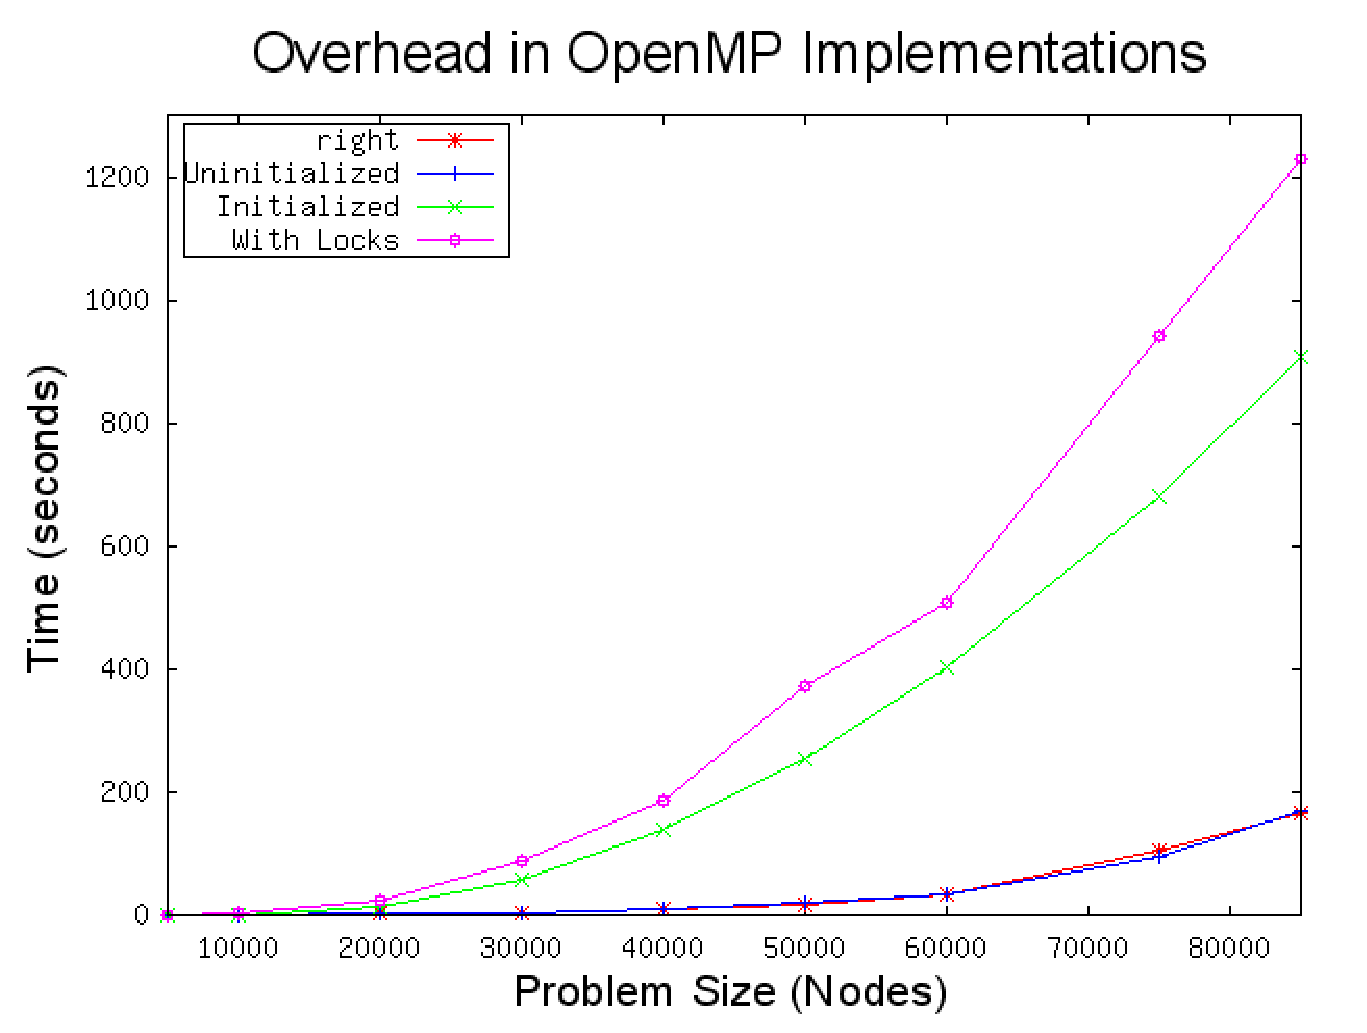
\includegraphics[width=0.75\textwidth]{images/figura1.eps}
\caption{Ejemplo de figura}
\label{fig:1}
\end{center}
\end{figure}
%------------------------------------------------------------------------------
\begin{table}[!ht]
\begin{center}
\begin{tabular}{|c|c|} \hline 
\textbf{Intento} & \textbf{Tiempo (segundos)} \\  \hline
1 & $2.8133*10^-5$ \\%Pidiendo el programa
2 & $2.4080*10^-5$ \\%Puestos directamente usuario
3 & $3.1948*10^-5$ \\%Puestos por consola e intervalo -10,10 
\hline
\end{tabular}
\end{center}
\caption{Tabla experimento 5}
\label{Mitabla5}
\end{table}


%------------------------------------------------------------------------------

%++++++++++++++++++++++++++++++++++++++++++++++++++++++++++++++++++++++++++++++
\section{An�lisis de los resultados}
\label{3:sec:4}

bla, bla, etc. 



%%%%%%%%%%%%%%%%%%%%%%%%%%%%%%%%%%%%%%%%%%%%%%%%%%%%%%%%%%%%%%%%%%%%%%%%%%%%%%%
\chapter{Conclusiones}
\label{chapter:conclusiones}

%%%%%%%%%%%%%%%%%%%%%%%%%%%%%%%%%%%%%%%%%%%%%%%%%%%%%%%%%%%%%%%%%%%%%%%%%%%%%
% Chapter 4: Conclusiones y Trabajos Futuros 
%%%%%%%%%%%%%%%%%%%%%%%%%%%%%%%%%%%%%%%%%%%%%%%%%%%%%%%%%%%%%%%%%%%%%%%%%%%%%%%

bla, bla, bla, etc.


%%%%%%%%%%%%%%%%%%%%%%%%%%%%%%%%%%%%%%%%%%%%%%%%%%%%%%%%%%%%%%%%%%%%%%%%%%%%%%%

%%%%%%%%%%%%%%%%%%%%%%%%%%%%%%%%%%%%%%%%%%%%%%%%%%%%%%%%%%%%%%%%%%%%%%%%%%%%%%%
\newpage{\pagestyle{empty}\cleardoublepage}
\thispagestyle{empty}
\begin{appendix}

\chapter{Algoritmos de bisecci�n y hardware y software}
\label{appendix:1}

\section{Algoritmo Metodo de Biseccion}
\label{Apendice1:Metodo de Biseccion}

\begin{center}
\begin{footnotesize}
\begin{verbatim}
#! /usr/bin/python
#!encoding: UTF-8
import time
import timeit

def f(x):
  return (5**x)-5
def biseccion(a,b,tol):
  c=(a+b)/2.0
  while((f(c)!=0.000001) and (abs(b-a)>tol)):
    if f(a)*f(c)<0.000001:
      b=c
    else:
      a=c
    c=(a+b)/2.0
  return c

import sys
if (len(sys.argv)==4):
  A=float(sys.argv[1])
  B=float(sys.argv[2])
  TOL=float(sys.argv[3]) 
else:
  A=float(raw_input("Introduzca el extremo a del intervalo: "))
  B=float(raw_input("Introduzca el extremo b del intervalo: "))
  TOL=float(raw_input("Introduzca la tolerancia del error que desee: "))
if f(A)*f(B)<0.000001:
  start=time.time()
  raiz=biseccion(A,B,TOL)
  finish=time.time()-start
  print "El tiempo de ejecucion es:"
  print finish
  print "La raiz aproximada de la funcion escogida es: %4.3f" %raiz
else:
  print "En ese intervalo no existe raíz, por favor vuelva a ejecutar el programa con otros valores"
\end{verbatim}
\end{footnotesize}
\end{center}

\section{Algoritmo Hardware y Software}
\label{Apendice1:Hardware y Software}

\begin{center}
\begin{footnotesize}
\begin{verbatim}

import os
import platform

def SOFTinfo():
  softinfo={}
  softinfo={'Several': platform.uname() , 'S.O':platform.platform(), 'Pythons Version': platform.python_version() , 'Date':platform.python_build()}
  return softinfo

def CPUinfo():
# infofile on Linux machines:
  infofile = '/proc/cpuinfo'
  cpuinfo = {}
  if os.path.isfile(infofile):
    f = open(infofile, 'r')
    for line in f:
      try:
	name, value = [w.strip() for w in line.split(':')]
      except:
	continue
      if name == 'model name':
	cpuinfo['CPU type'] = value
      elif name == 'cache size':
	cpuinfo['cache size'] = value
      elif name == 'cpu MHz':
	cpuinfo['CPU speed'] = value + 'Hz'
      elif name == 'vendor_id':
	cpuinfo['vendor ID'] = value
    f.close()
  return cpuinfo

if __name__ == '__main__':
  
  softinfo=SOFTinfo()
  for keys in softinfo.keys():
    print softinfo[keys]
    
  cpuinfo=CPUinfo()
  for keys in cpuinfo.keys():
    print CPUinfo()
  
  print "Introduzca el nombre del fichero para almacenar los resultados:"
  nombre_fichero= raw_input();
  f=open(nombre_fichero, "w")
  
  for keys in softinfo.keys():
    if type (softinfo[keys]) is list:
      f.write('\n'.join(softinfo[keys]))
    else:
      f.write(str(softinfo[keys]))
      f.write('\n')
      
  for keys in cpuinfo.keys():
    if type (cpuinfo[keys]) is list:
      f.write('\n'.join(cpuinfo[keys]))
    else:
      f.write(str(cpuinfo[keys]))
      f.write('\n')
  f.close()
\end{verbatim}
\end{footnotesize}
\end{center}


\chapter{Algoritmos de gr�ficas}
\label{appendix:2}

\section{Otro apendice: Seccion 1}
\label{Apendice2:label}

\begin{center}
\begin{footnotesize}

\begin{verbatim}
Texto
\end{verbatim}

\end{footnotesize}
\end{center}

\section{Otro apendice: Seccion 2}
\label{Apendice2:label2}

\begin{center}
\begin{footnotesize}

\begin{verbatim}
Texto
\end{verbatim}


\end{footnotesize}
\end{center}


\end{appendix}

%%%%%%%%%%%%%%%%%%%%%%%%%%%%%%%%%%%%%%%%%%%%%%%%%%%%%%%%%%%%%%%%%%%%%%%%%%%%%%%
\addcontentsline{toc}{chapter}{Bibliograf�a}
\bibliographystyle{plain}

\input{tex/biblio.tex}
%\bibliography{bib/references}
\nocite{*}

%%%%%%%%%%%%%%%%%%%%%%%%%%%%%%%%%%%%%%%%%%%%%%%%%%%%%%%%%%%%%%%%%%%%%%%%%%%%%%%

\end{document}
